\section{Environment specification, Invasive Species}
\label{sec:experiment_env}

When the agents were tested, the Invasive Species environment from the 2014 edition of
the Reinforcement Learning Competition was used. The environment is a
simulation of an invasive species problem, in this case a river network where the goal of the agent is to eradicate unwanted species
while replanting native species. 

The environment's model of the river network has parameters, such as the size
of the river network and the rate at which plants spread, which can be
configured in order to create different variations of the environment.  The
size of the river network is defined by two parameters: the number of reaches
and the number of habitats per reach. A habitat is the smallest unit of land
that is considered in the problem. A habitat can either be invaded by the
tamarix, which is an unwanted species, empty or occupied by native species. A
reach is a collection of neighboring habitats. The structure of the river
network is defined in terms of which reach is connected to which
\parencite{invasiveSpecis2014:Online}. In figure \ref{fig:river} a model of a
river network is shown.

\begin{figure}[ht]
\centering
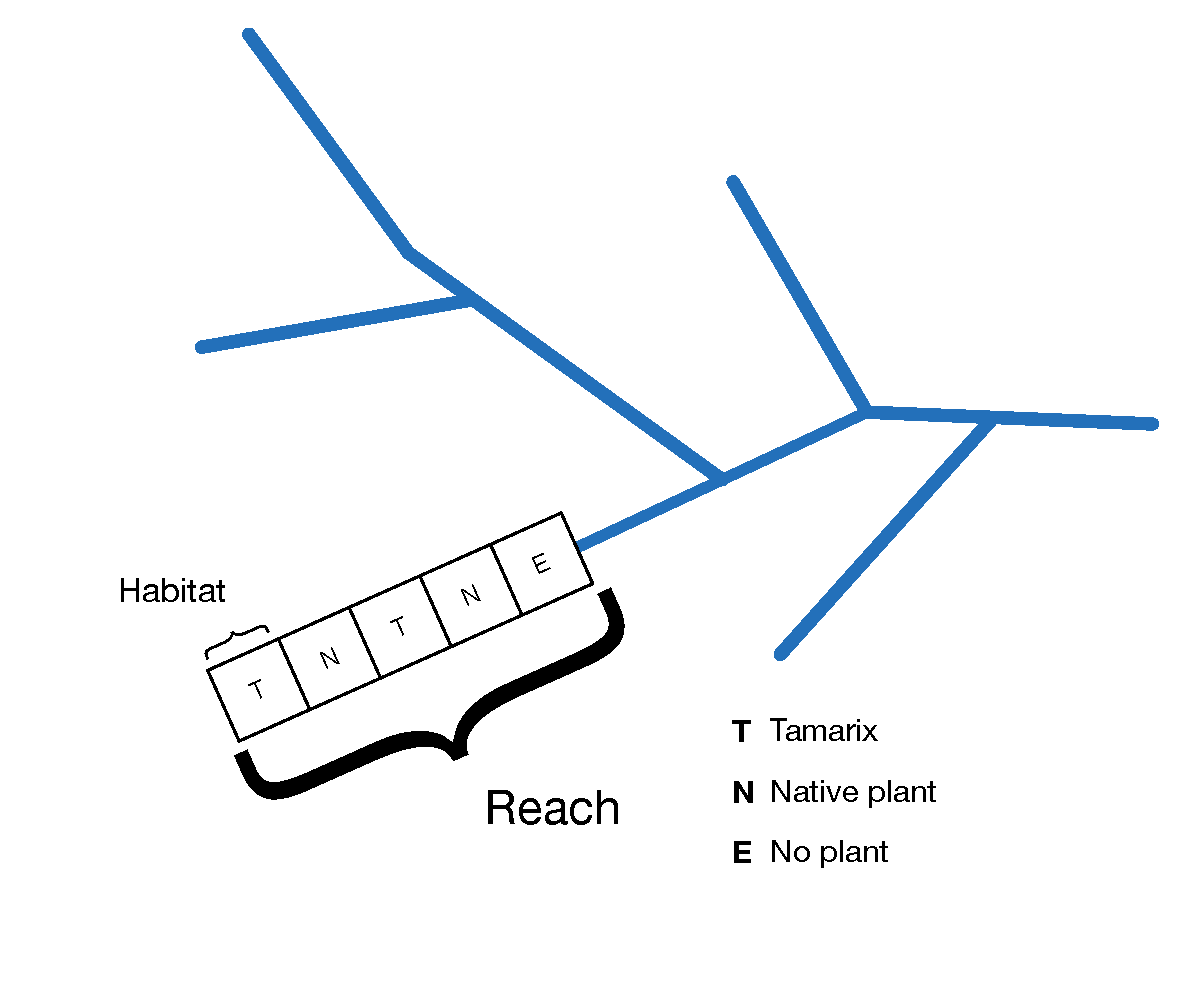
\includegraphics[width=0.9\textwidth]{images/river_network.pdf}
\caption{A river network, as modeled by the Invasive Species reinforcement learning environment.}
\label{fig:river}
\end{figure}

There are four possible actions (eradicate tamarix trees, plant native trees,
eradicate tamarix trees and plant native trees and a wait-and-see action),
and the agent chooses one of these actions for each reach and time step. If the 
agent chooses to eradicate tamarix trees or plant native trees in a reach, 
all habitats of that reach are targeted by this action. What
actions are available to the agent depends on the state of each reach. It is
always possible to choose the wait-and-see action, but there has to be one
or more tamarix-invaded habitats in a reach for the eradicate or eradicate and
plant actions to be available and there has to be at least one empty habitat in
a reach for the plant-native-trees action to be available
\parencite{invasiveSpecis2014:Online}.  
